% TEX program = xelatex
% TEX encoding = UTF-8

\documentclass[article, a4paper, 12pt]{memoir}

\usepackage{silence}
\WarningsOff[biblatex]

\usepackage{fontspec}
\usepackage[main=english]{babel}

\setmainfont[BoldFont={Brill Bold},ItalicFont={Brill Italic}]{Brill}
\setmonofont[Scale=0.75]{Noto Mono}

\usepackage{linguex}
\usepackage{tikz} %for all basic options
\usepackage{tikz-qtree} %for simple tree syntax
\usepgflibrary{arrows} %for arrow endings
\usetikzlibrary{positioning,shapes.multipart} %for structured nodes
\usetikzlibrary{tikzmark}
\usepackage{tikz-qtree}
\usepackage{tree-dvips}
\usepackage{xargs}
\usepackage{booktabs}
\usepackage{tabularx}
\usepackage[normalem]{ulem}

% Pacotes de diagramação
\usepackage{paralist}
\usepackage{longtable}
\usepackage{multirow}
\usepackage{amsmath}
\usepackage{amsfonts}
\usepackage{graphicx}
\usepackage{hyphenat}

\usepackage{hyperref}
\usepackage{bookmark}
\usepackage{listings}

\author{Caio Borges Aguida Geraldes}
\title{Week 9 --- Homework}
\date{\today}

\usepackage[backend=biber,
            style=abnt,
            pretty,
            repeatfields,
            noslsn,
            natbib,
            extrayear,
            ]{biblatex}
\addbibresource{~/.biblio.bib}

\DeclareMathOperator{\logit}{logit}
\DeclareMathOperator{\normal}{Normal}
\DeclareMathOperator{\exponential}{Exponential}
\DeclareMathOperator{\binomial}{Binomial}
\DeclareMathOperator{\bernoulli}{Bernoulli}

\definecolor{codegreen}{rgb}{0,0.6,0}
\definecolor{codegray}{rgb}{0.5,0.5,0.5}
\definecolor{codepurple}{rgb}{0.58,0,0.82}
\definecolor{backcolor}{rgb}{0.95,0.95,0.92}

\lstdefinestyle{mystyle}{%
    backgroundcolor=\color{backcolor},
    commentstyle=\color{codegreen},
    keywordstyle=\color{magenta},
    numberstyle=\tiny\color{codegray},
    stringstyle=\color{codepurple},
    basicstyle=\ttfamily\footnotesize,
    breakatwhitespace=false,
    breaklines=true,
    captionpos=b,
    keepspaces=true,
    numbers=left,
    numbersep=5pt,
    showspaces=false,
    showstringspaces=false,
    showtabs=false,
    tabsize=2
}

\lstset{style=mystyle}

\usepackage[backend=biber,
            style=abnt,
            pretty,
            repeatfields,
            noslsn,
            natbib,
            extrayear,
            ]{biblatex}
\addbibresource{biblio.bib}

\begin{document}

\maketitle

\chapter*{Previous assumptions}

As it will become important to our theoretical model, it must be noted that the data in~\textcite{HillKintigh2009} has been collected from 1980 to 2007 by two different means: observational (1980--2000) and by interviews (1994--2007).
Notice also that there are no data points for the years 1986 to 1993.
Whereas the authors argue that the data for kilograms of meat and the hunter\hyp{}dependent information, the number of hours for each hunting trip was not consistently recorded, as shown in~\autoref{fig:missing}.

\begin{figure}[!htb]
\begin{center}
    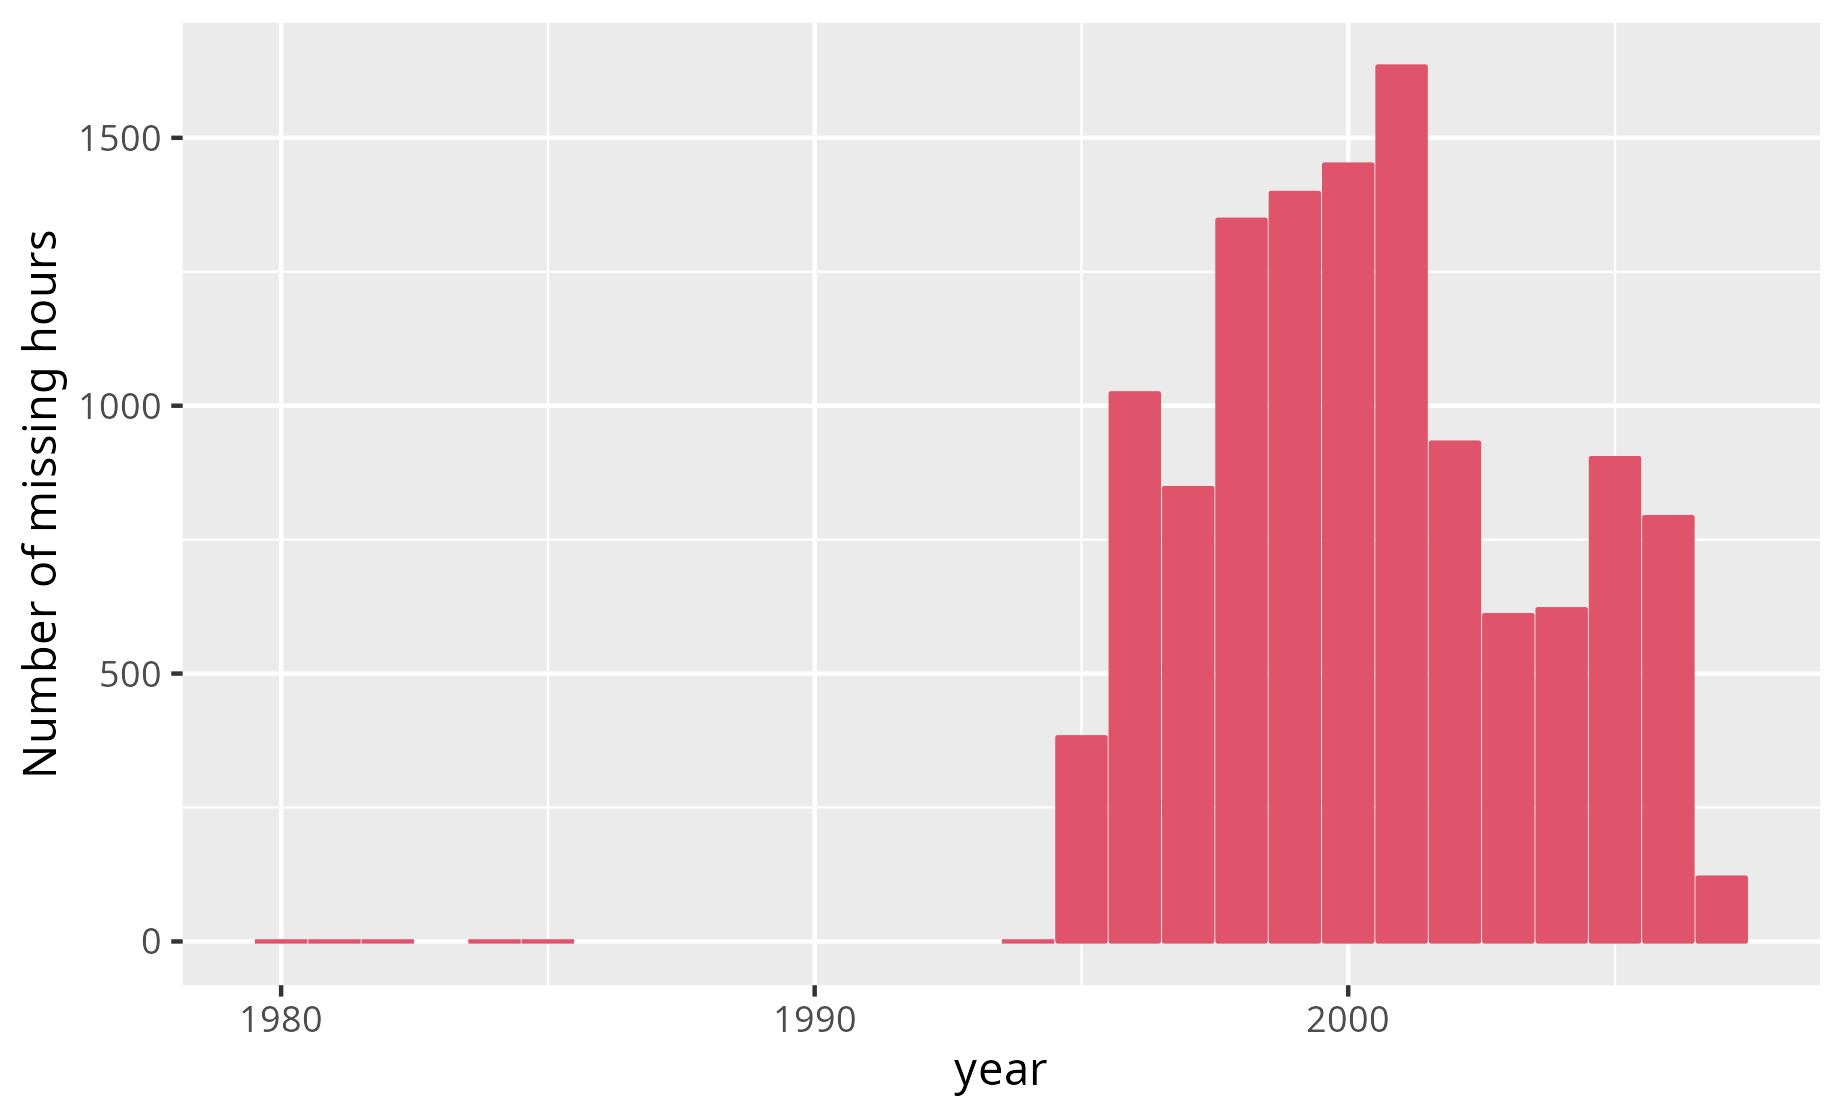
\includegraphics[width=0.75\textwidth]{./plots/missing.png}
\end{center}
\caption{Count of missing data for hours expend hunting by year.}\label{fig:missing}
\end{figure}

As a consequence, the scientific model must account for year, in some measure, as the variable $T$ is unobserved, and the hours actually observed $T^*$ are dependent on year.
Hunter $H$, age $A$, and time $T$ will affect the likelihood of scoring a game in a hunting trip.
The DAG of the model assumed will be:

\begin{center}
    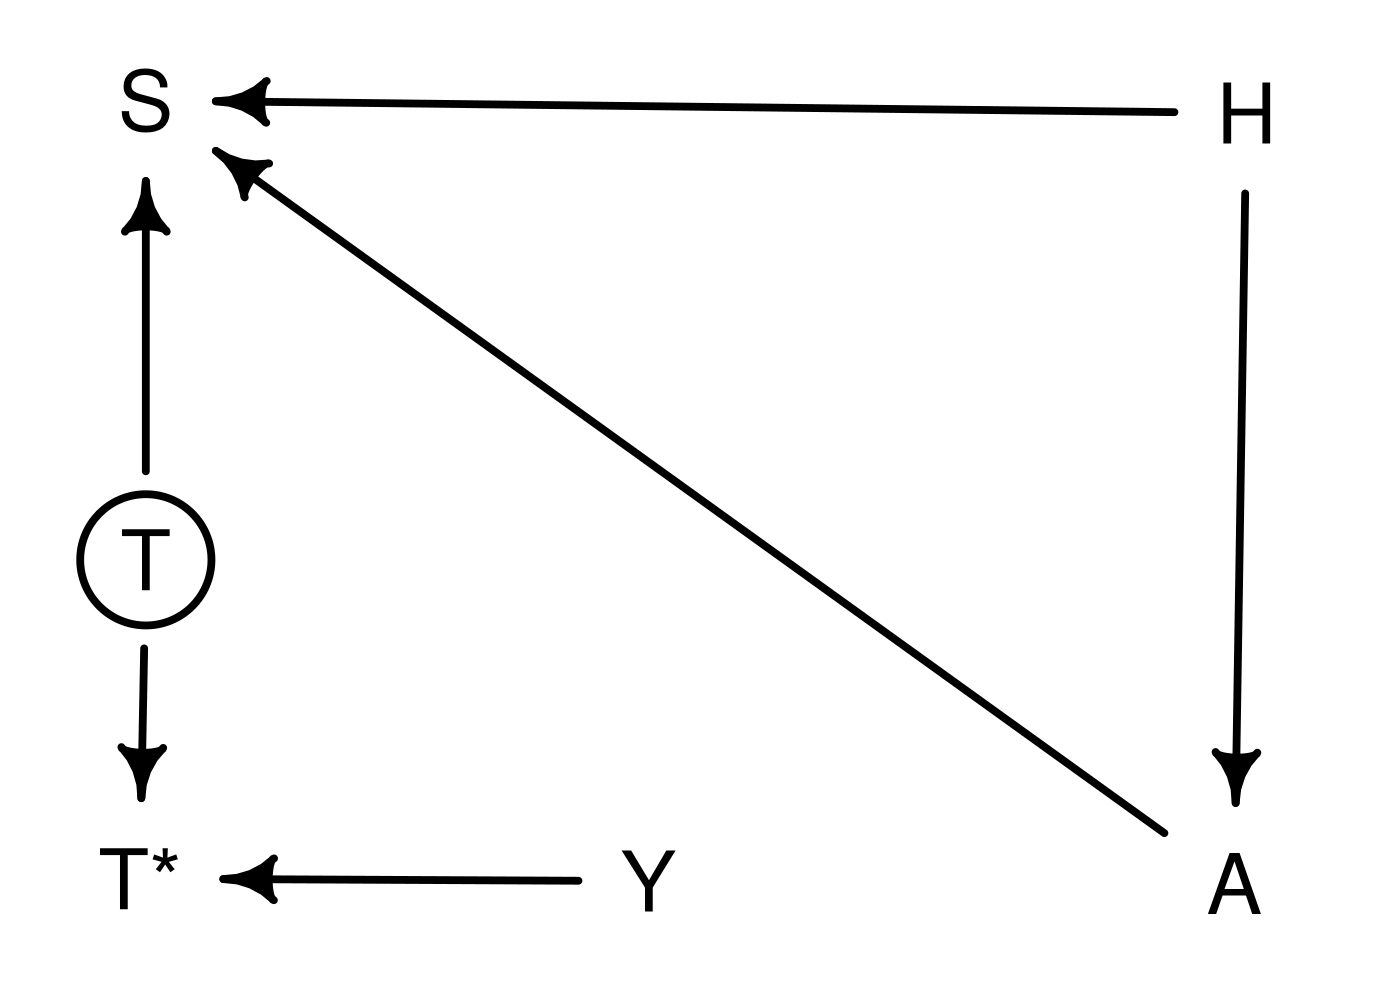
\includegraphics[width=0.5\textwidth]{./plots/dag.png}
\end{center}


\chapter*{Exercice 1}

Assuming that all the Aché individuals in the data \texttt{Achehunting} are functionally adults (as they seem to take active part in the tasks for sustaining their community), we can suppose that their age will affect their hunting success in a quadratic way:
young adults will be still learning how to hunt properly, whereas older members of the community will gradually loose their ability to hunt effectively.
I model the effect of age over hunting success as a quadratic linear model, where $\alpha$ denotes the average likelihood of any member of the community to successfully come back from a hunting trip with some game, and $\beta$ the effect of z\hyp{}score of age squared:

\begin{equation*}
    \logit(p) = \alpha + \beta A_i^2
\end{equation*}

As the success of any hunting trip $i$, $S_i$, is true or false, it is modeled as a $\bernoulli$ distribution on $p_i$:

\begin{align*}
    S_i& \sim \bernoulli(p_i)\\
    \logit(p_i)& = \alpha + \beta A_i^2
\end{align*}

I pick very flat priors that favour values of $\beta \leq 0$, so the final model is:

\begin{align*}
    S_i& \sim \bernoulli(p_i)\\
    \logit(p_i)& = \alpha + \beta A_i^2\\
    \alpha& \sim \normal(0,0.1)\\
    \beta& \sim \normal(0, 0.05)
\end{align*}

The model is processed by \texttt{ulam} and stored in a model file \texttt{models/mA.rds}:

\lstinputlisting[language=R, firstline=20, lastline=27]{./Geraldes-week9.R}

The precis table shows that $\beta$ is, as expected, consistently negative.
The whole distribution of $\beta$ is shown in~\autoref{fig:b.posterior.mA}.

\lstinputlisting[language=R, firstline=31, lastline=34]{./Geraldes-week9.R}


\begin{figure}[!hbt]
\begin{center}
    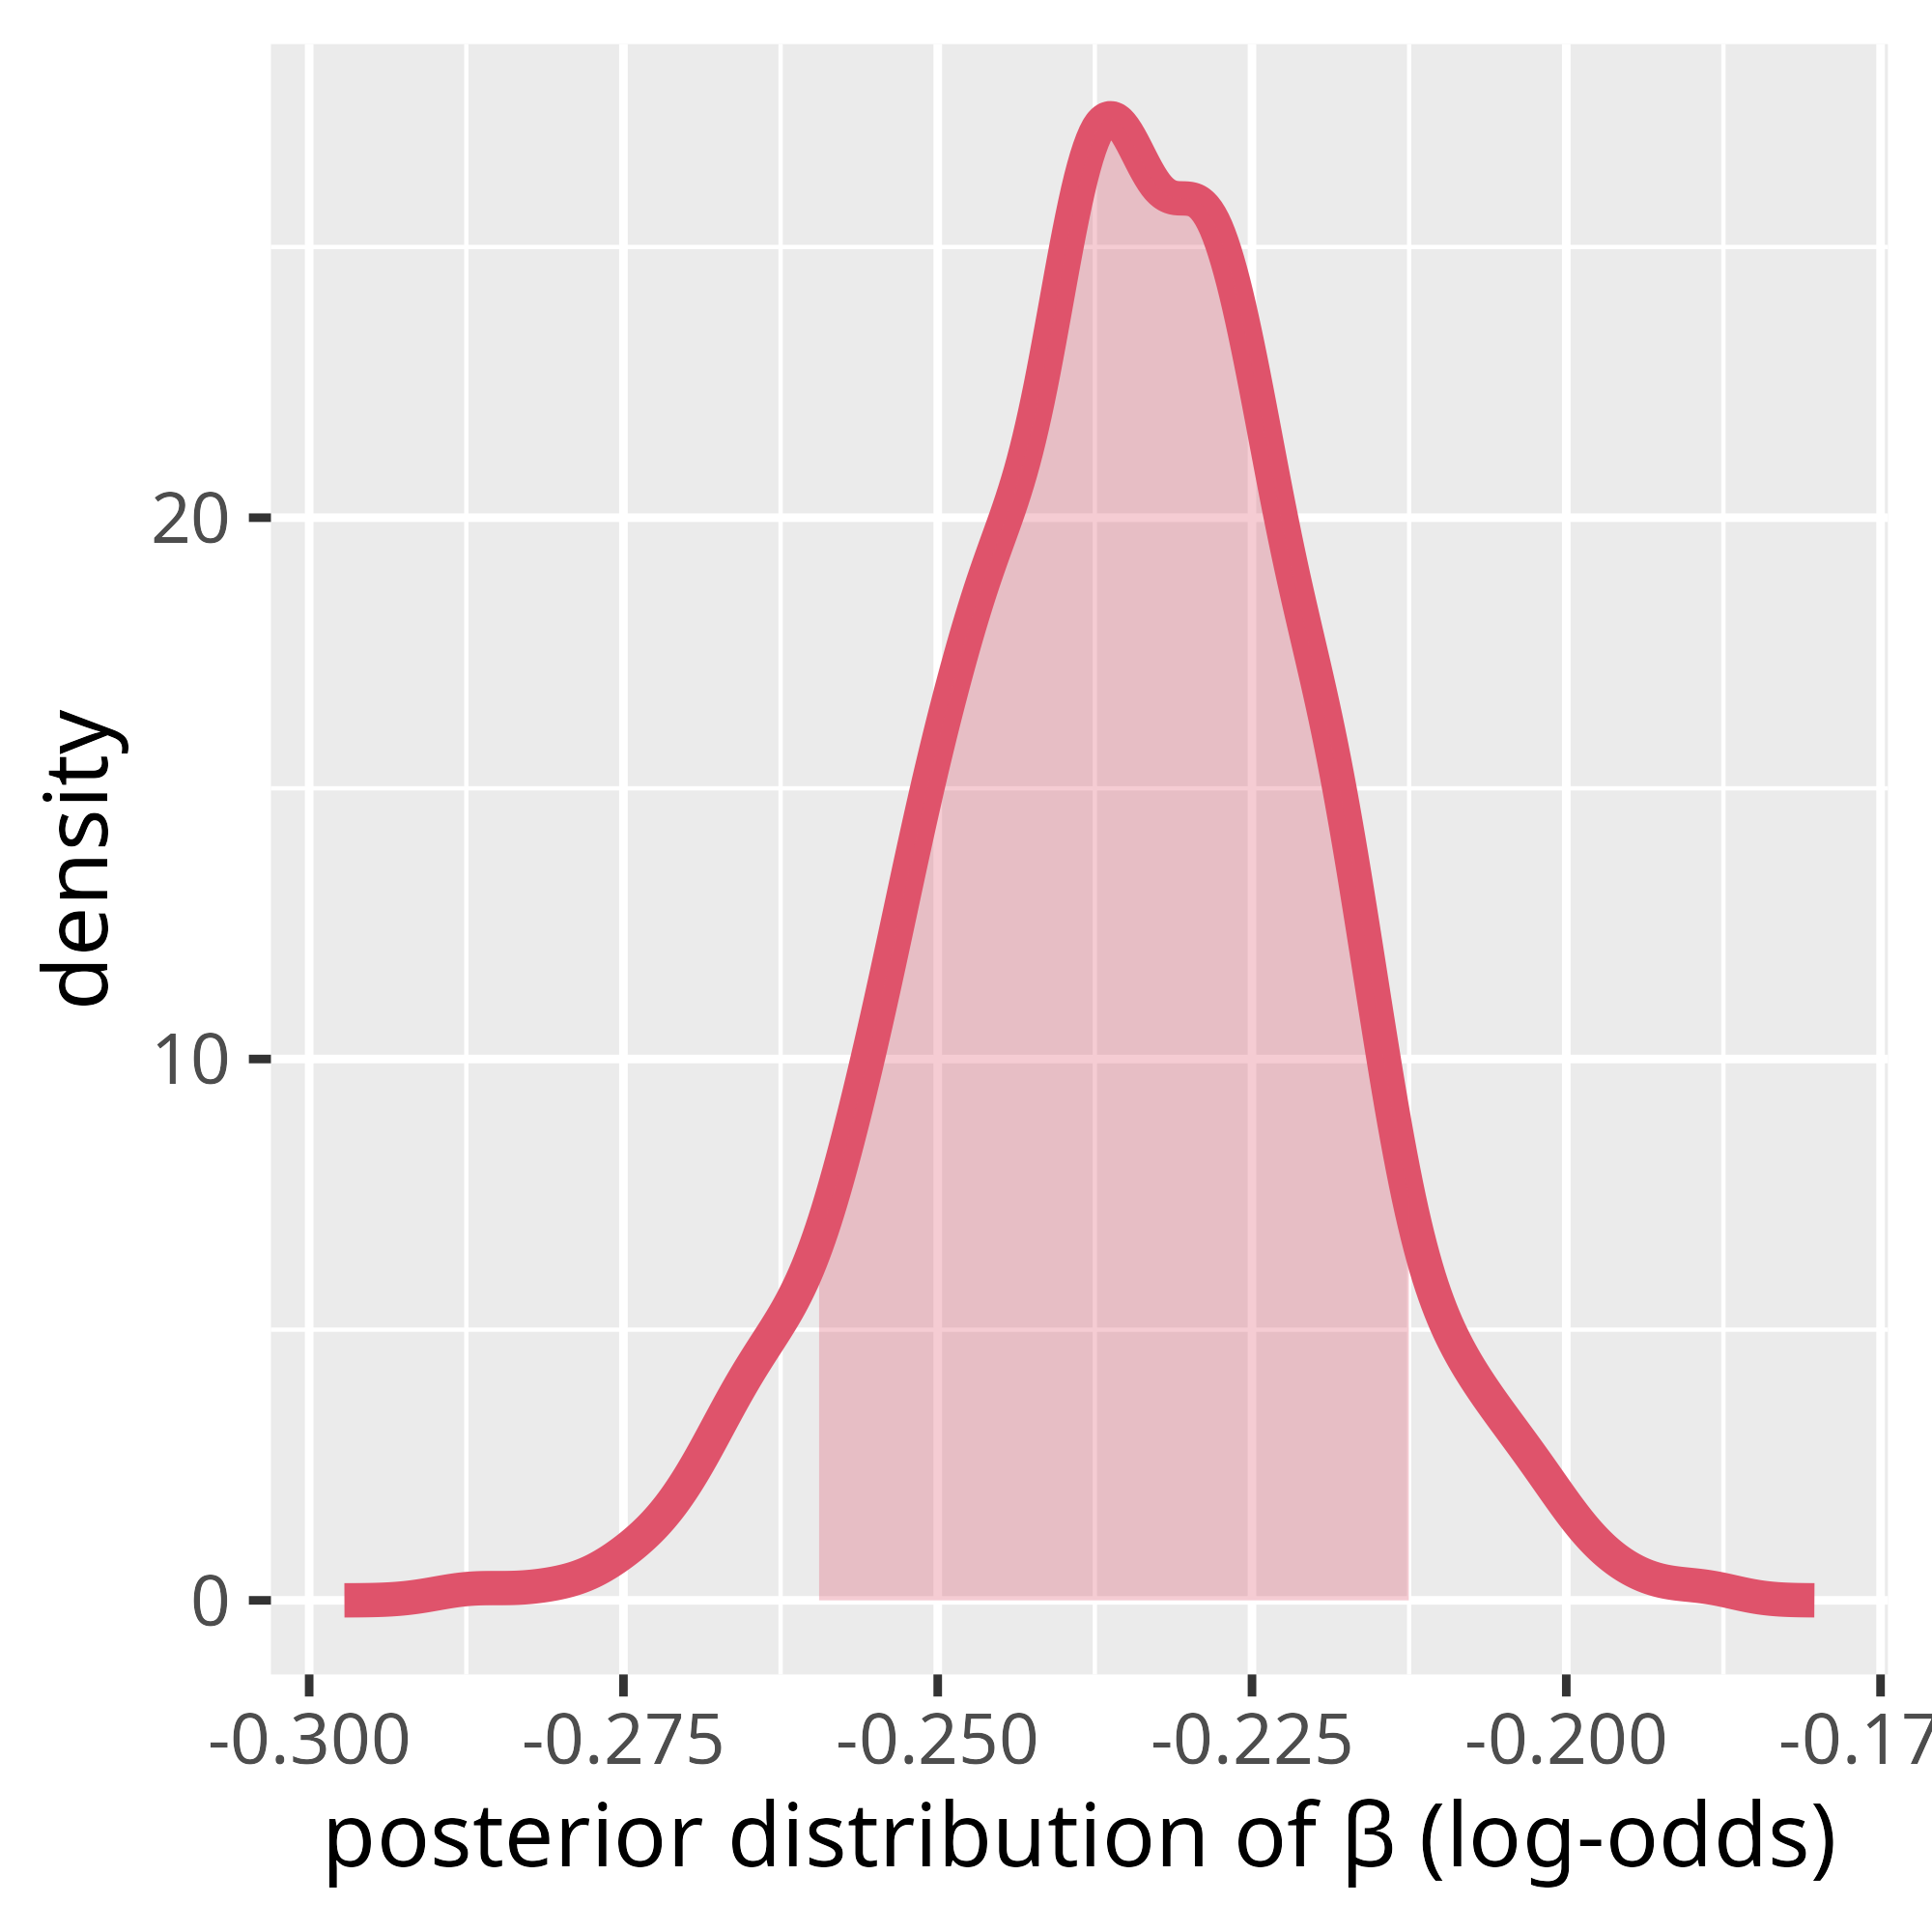
\includegraphics[width=0.5\textwidth]{./plots/b.posterior.mA.png}
\end{center}
\caption{Posterior distribution of $\beta$ with the 89\% HPDI compatibility interval shown in the red area.}\label{fig:b.posterior.mA}
\end{figure}

Using the predictive posterior distribution of the probabilities of returning with some game after a hunting trip, we can compare the model results with the data,~\autoref{fig:p.posterior.mA}.
The model has a lot of recall, particularly in the cases of individuals of lower age, as they seem to have not taken part on many hunting trips (hunters of age 11, 12 and 13 have only 1, 9 and 4 hunts recorded in total), so there is not enough data to see their real chances of having a successful hunt.

\begin{figure}[!htb]
\begin{center}
    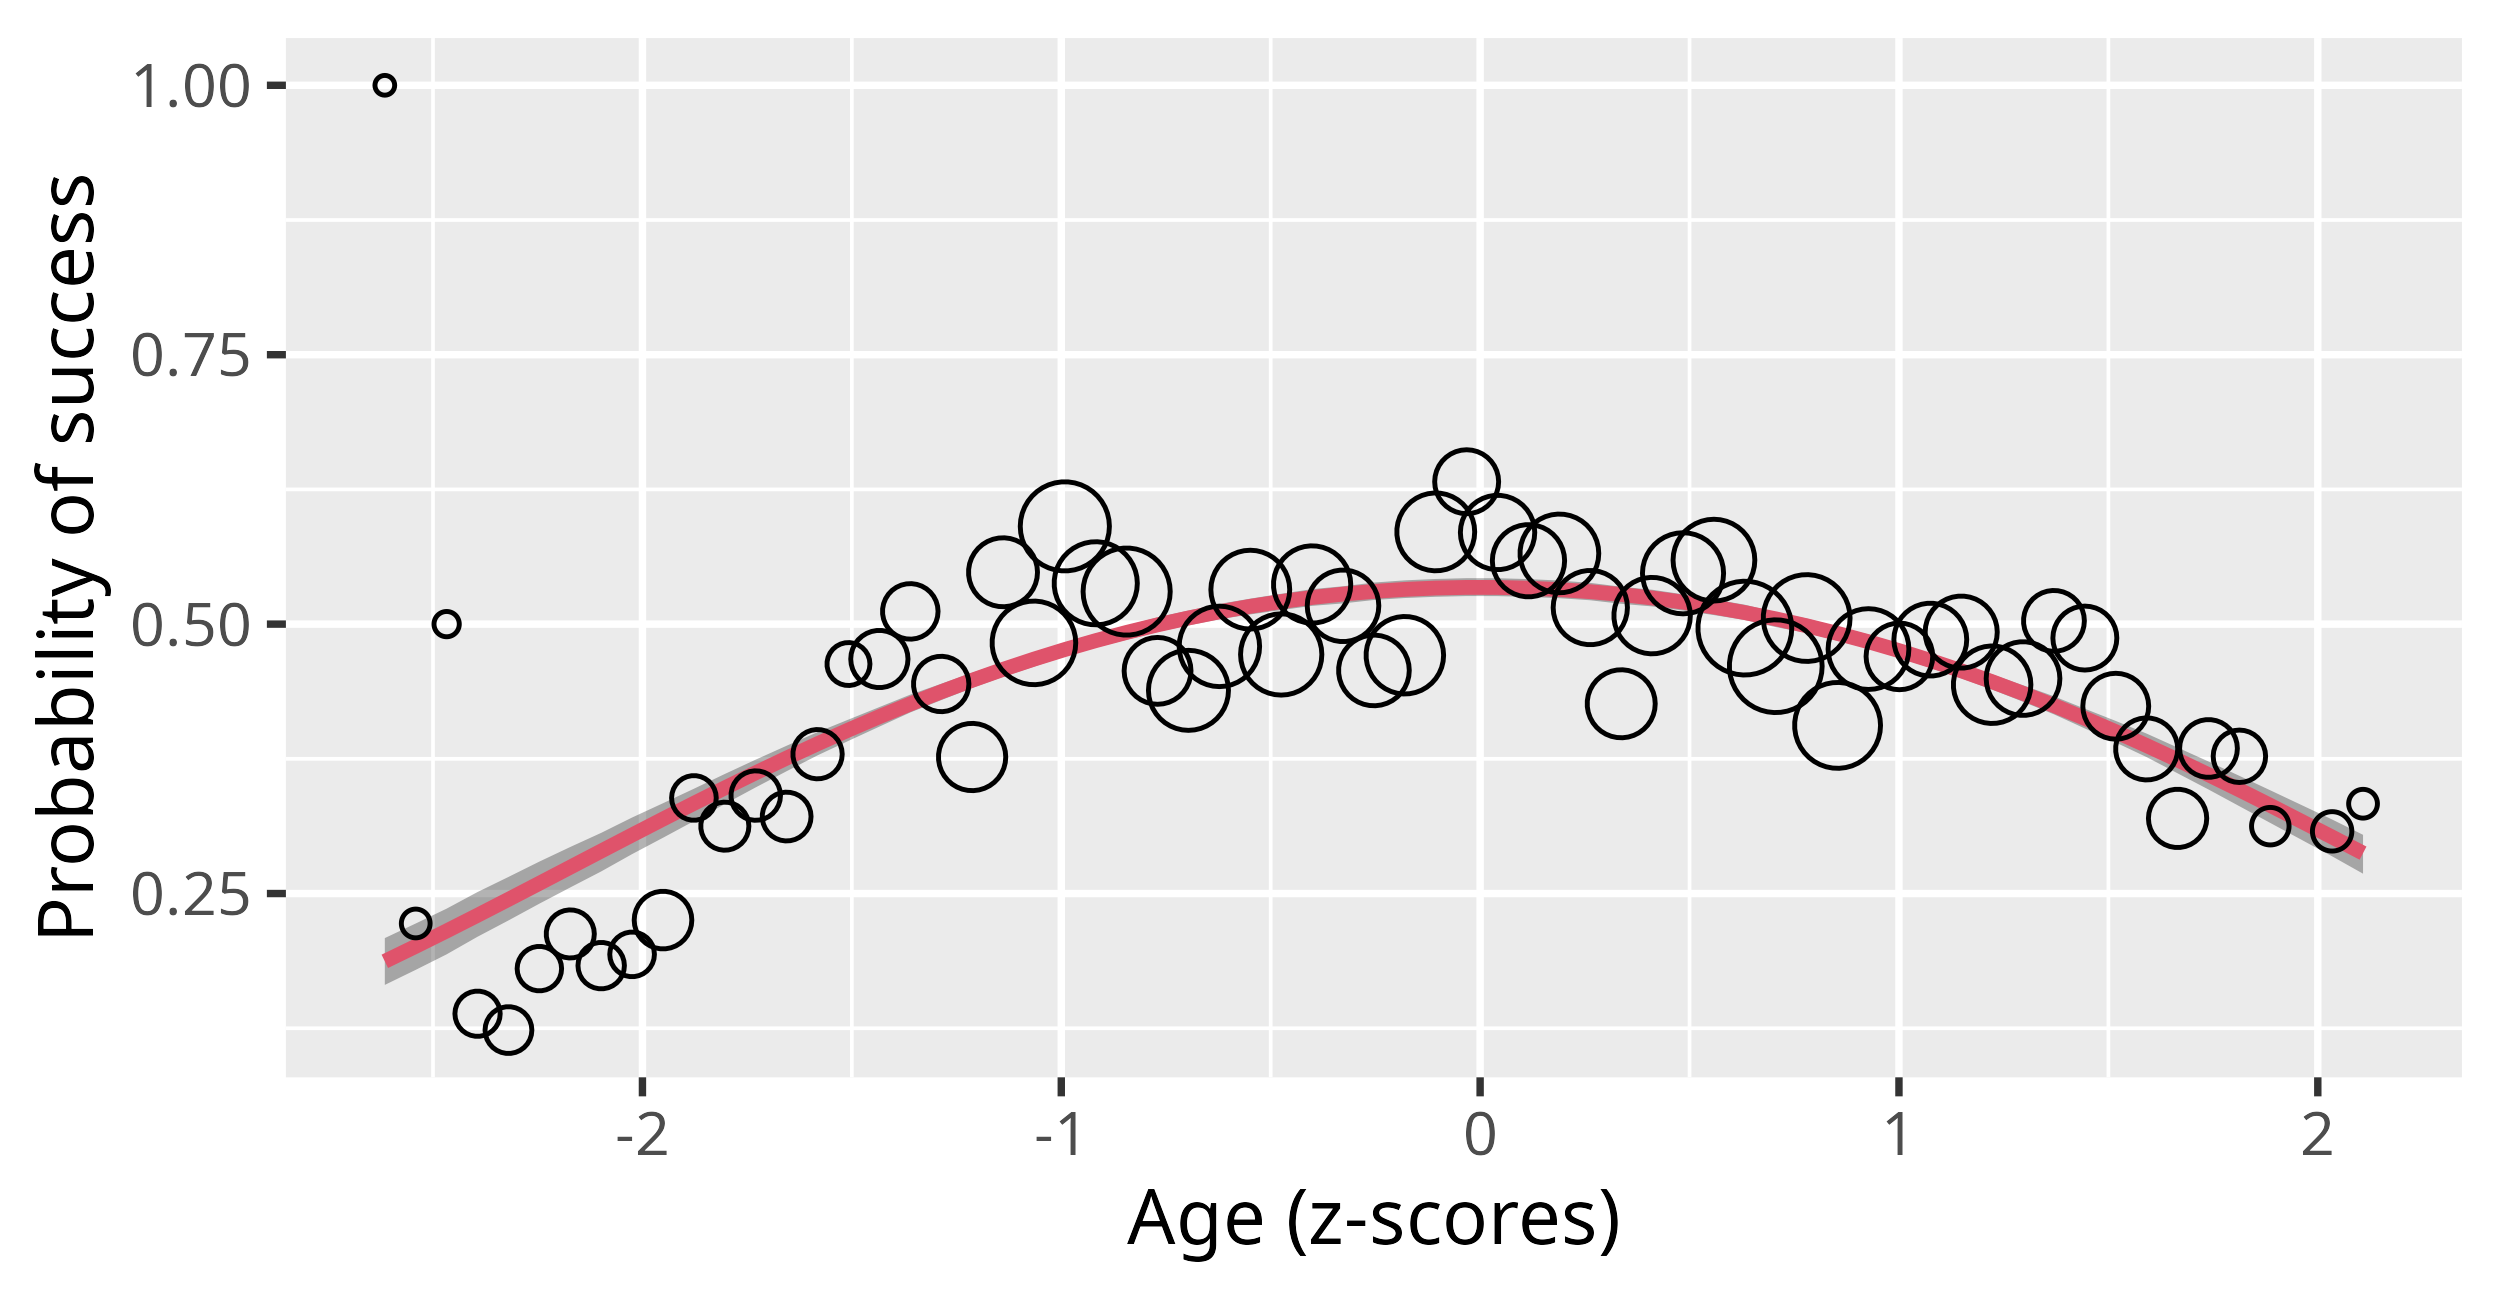
\includegraphics[width=\textwidth]{./plots/p.posterior.mA.png}
\end{center}
\caption{Posterior predictive distribution. The number of documented hunting trips per age is represented by the size of the points. The curve indicates the mean of the predictive posterior distribution with the 89\% HPDI compatibility interval.}\label{fig:p.posterior.mA}
\end{figure}

\chapter*{Exercice 2}

Assuming that each hunter $H$ has their own intercept, representing their physical and mental characteristics that affect their likelihood of scoring some game by each hunting trip they take, I change the previous parameter $\alpha$ to vary according to the hunter $H$, $\alpha_H$.
This parameter is partially pooled from the whole community of hunters, so that there is an average likelihood for any hunter to have a successful hunting trip, $\bar{\alpha}$, which is summed to an individual effect. I repeat the prior for $\alpha$ from the previous model as $\bar{\alpha}$ and build an non-centered distribution for the individual effects:

\begin{align*}
    \alpha_H& = \bar{\alpha} + z_{\alpha,H}\sigma_\alpha\\
    \bar{\alpha}& \sim \normal(0, 0.1)\\
    z_{\alpha,H}& \sim \normal(0,1)\\
    \sigma_\alpha& \sim \exponential(1)
\end{align*}

I include a non-centered parametrization also for $\beta$, so that $\beta = z_\beta\sigma_\beta$. The complete model used is as follows:

\begin{alignat*}{2}
    S_i& \sim \bernoulli(p_i)&\\
    \logit(p_i)& = \alpha_{H_i} + \beta A_i^2&\\
    \alpha_j& = \bar{\alpha} + z_{\alpha,j}\sigma_\alpha{}& \text{for $j = 1 \dots 147$}\\
    z_{\alpha,j}& \sim \normal(0,1)&\\
    \bar{\alpha}& \sim \normal(0, 0.1)&\\
    \sigma_\alpha& \sim \exponential(1)&\\
    \beta& = z_{\beta}\sigma_\beta&\\
    z_{\beta}& \sim \normal(0,1)&\\
    \sigma_\beta& \sim \exponential(1)&
\end{alignat*}


The model is processed by \texttt{ulam} and stored in a model file \texttt{models/mAI.rds}:

\lstinputlisting[language=R, firstline=45, lastline=57]{./Geraldes-week9.R}

The precis table for the fitted model:

\lstinputlisting[language=R, firstline=61, lastline=67]{./Geraldes-week9.R}

Comparing to the previous model, the effect of age is overall lower and has more variation, so that stronger and weaker effects are possible.
The effect is still negative, as expected.
See~\autoref{fig:p.posterior.mAI}.
The effect of the individual $\alpha_H$ still has a lot of variation depending on how many trips were documented for that particular individual.
See~\autoref{fig:p.posterior.mAI2}.

\begin{figure}[!htb]
\begin{center}
    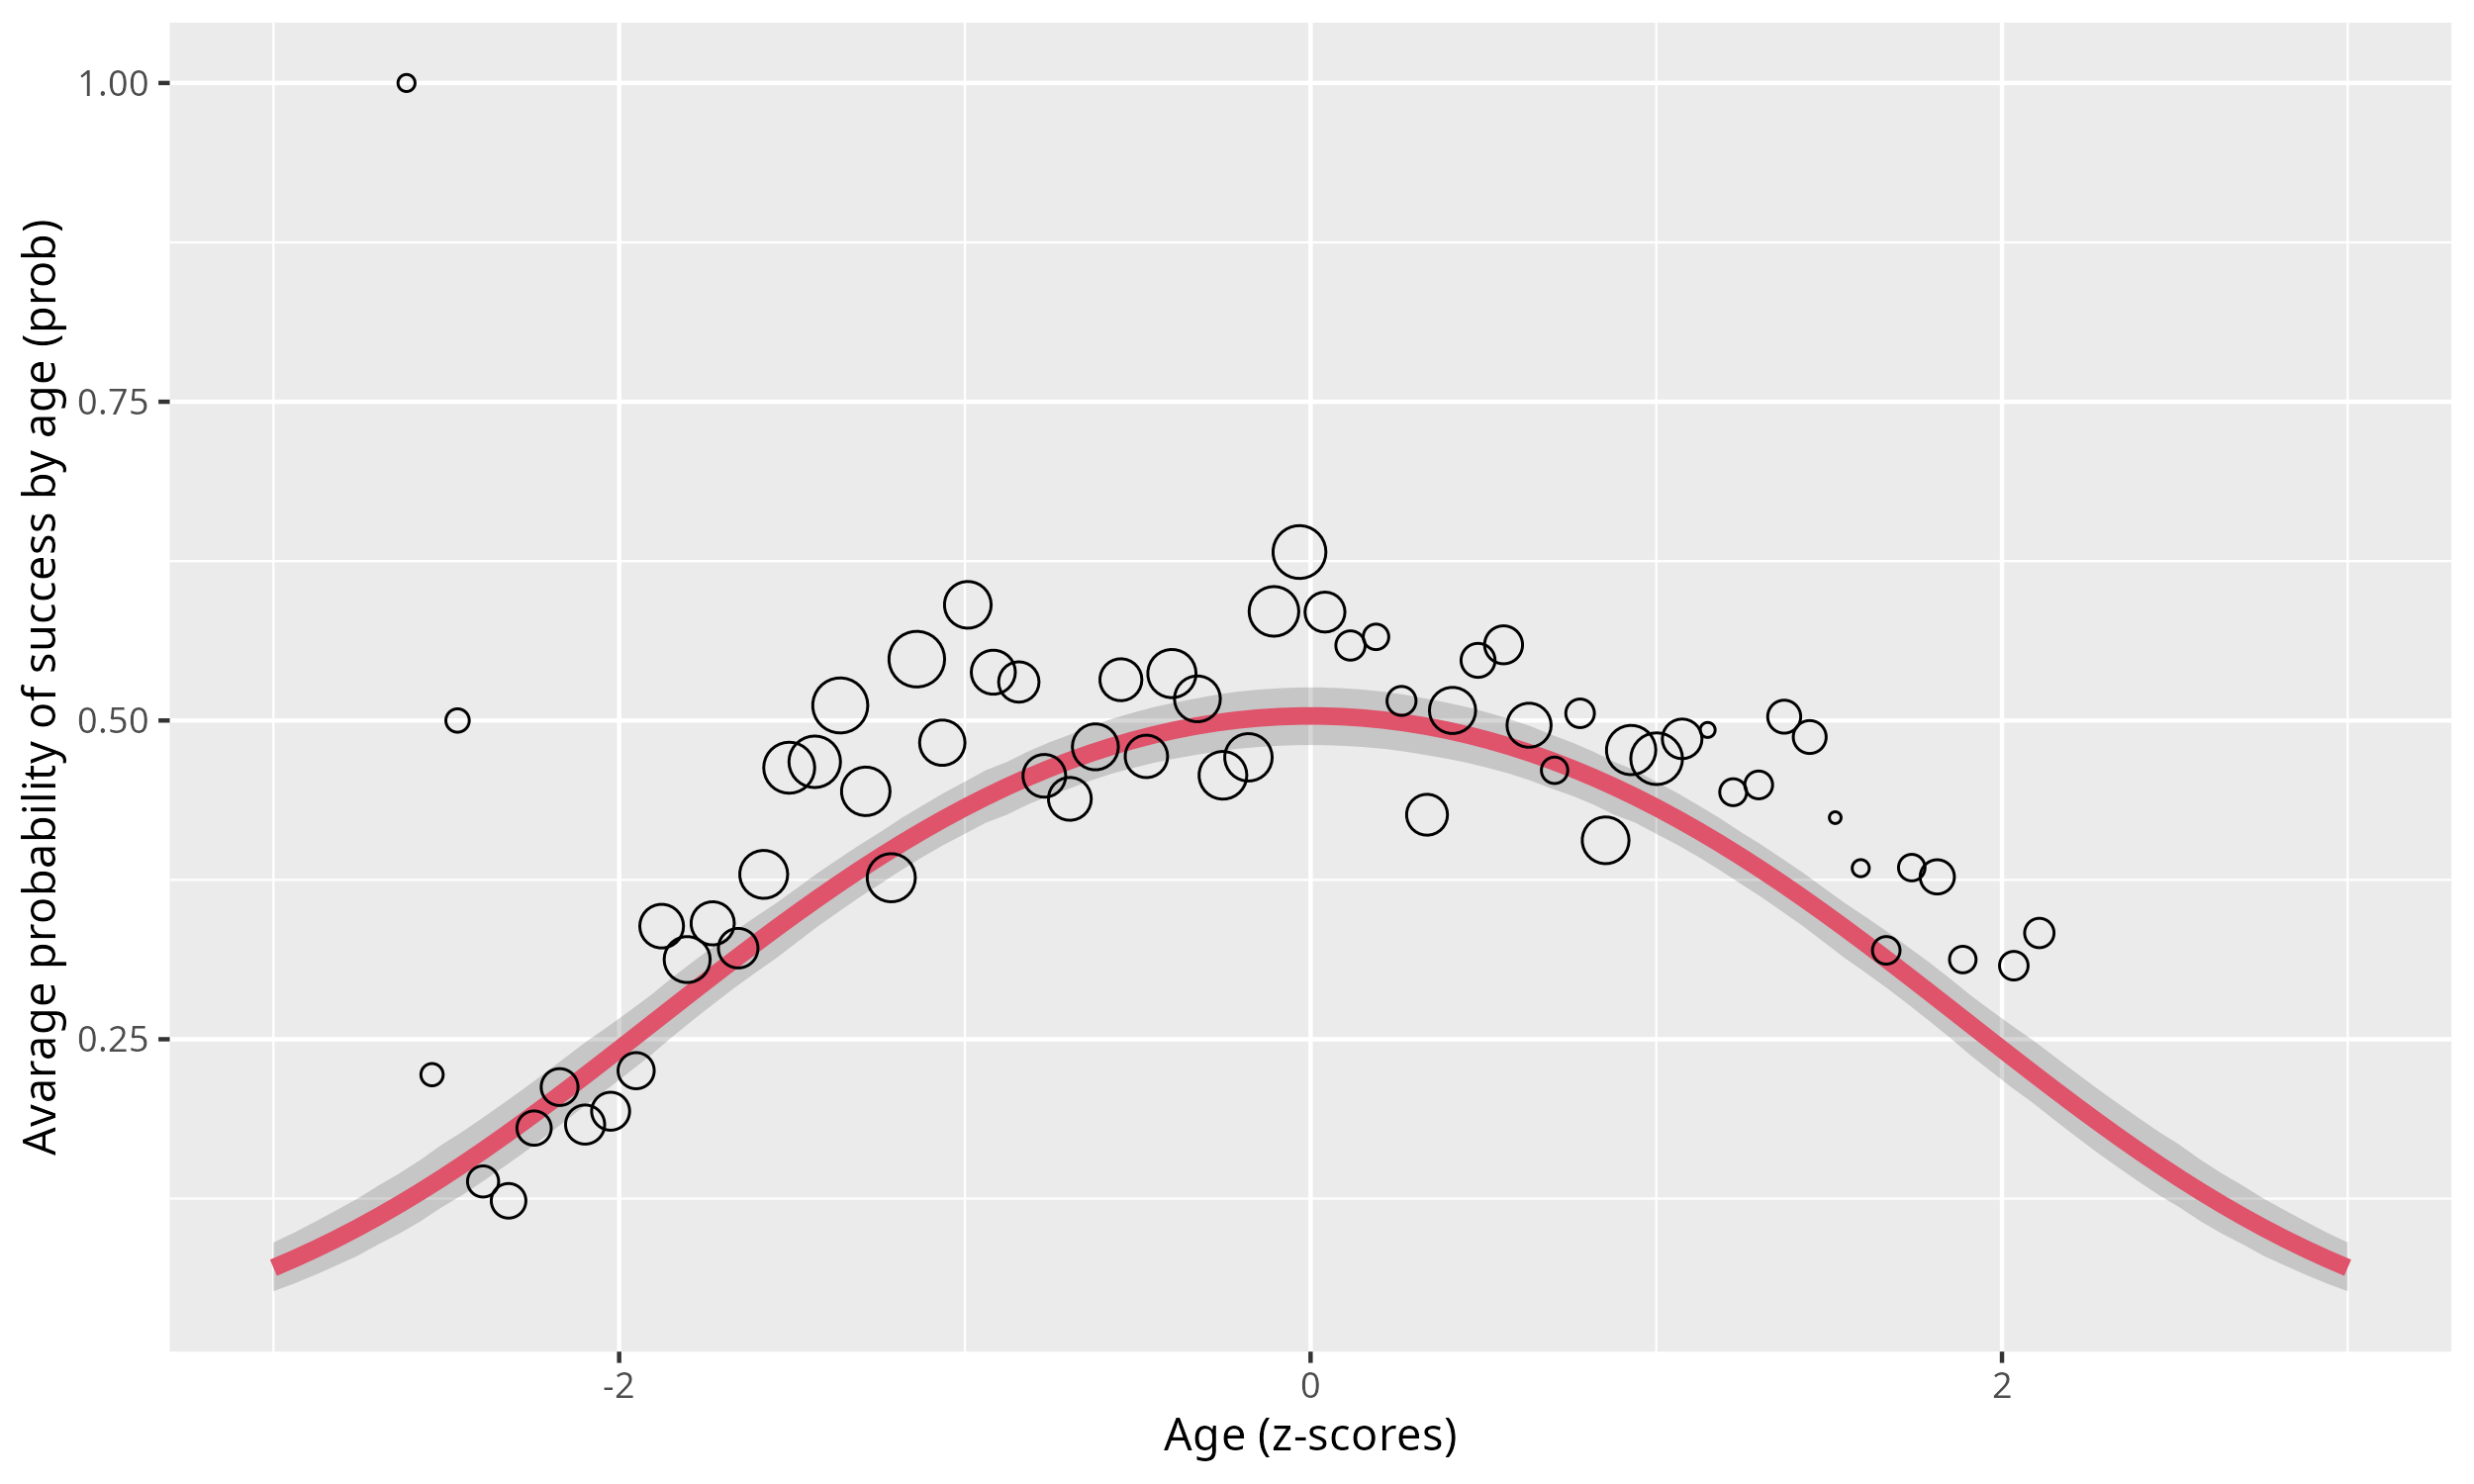
\includegraphics[width=1\textwidth]{./plots/p.posterior.mAI.png}
\end{center}
\caption{Posterior predictive distribution, marginalized over individuals (using $\bar{\alpha}$ in the link function). The number of documented hunting trips per age is represented by the size of the points. The curve indicates the mean of the predictive posterior distribution with the 89\% HPDI compatibility interval.}\label{fig:p.posterior.mAI}
\end{figure}

\begin{figure}[!htb]
\begin{center}
    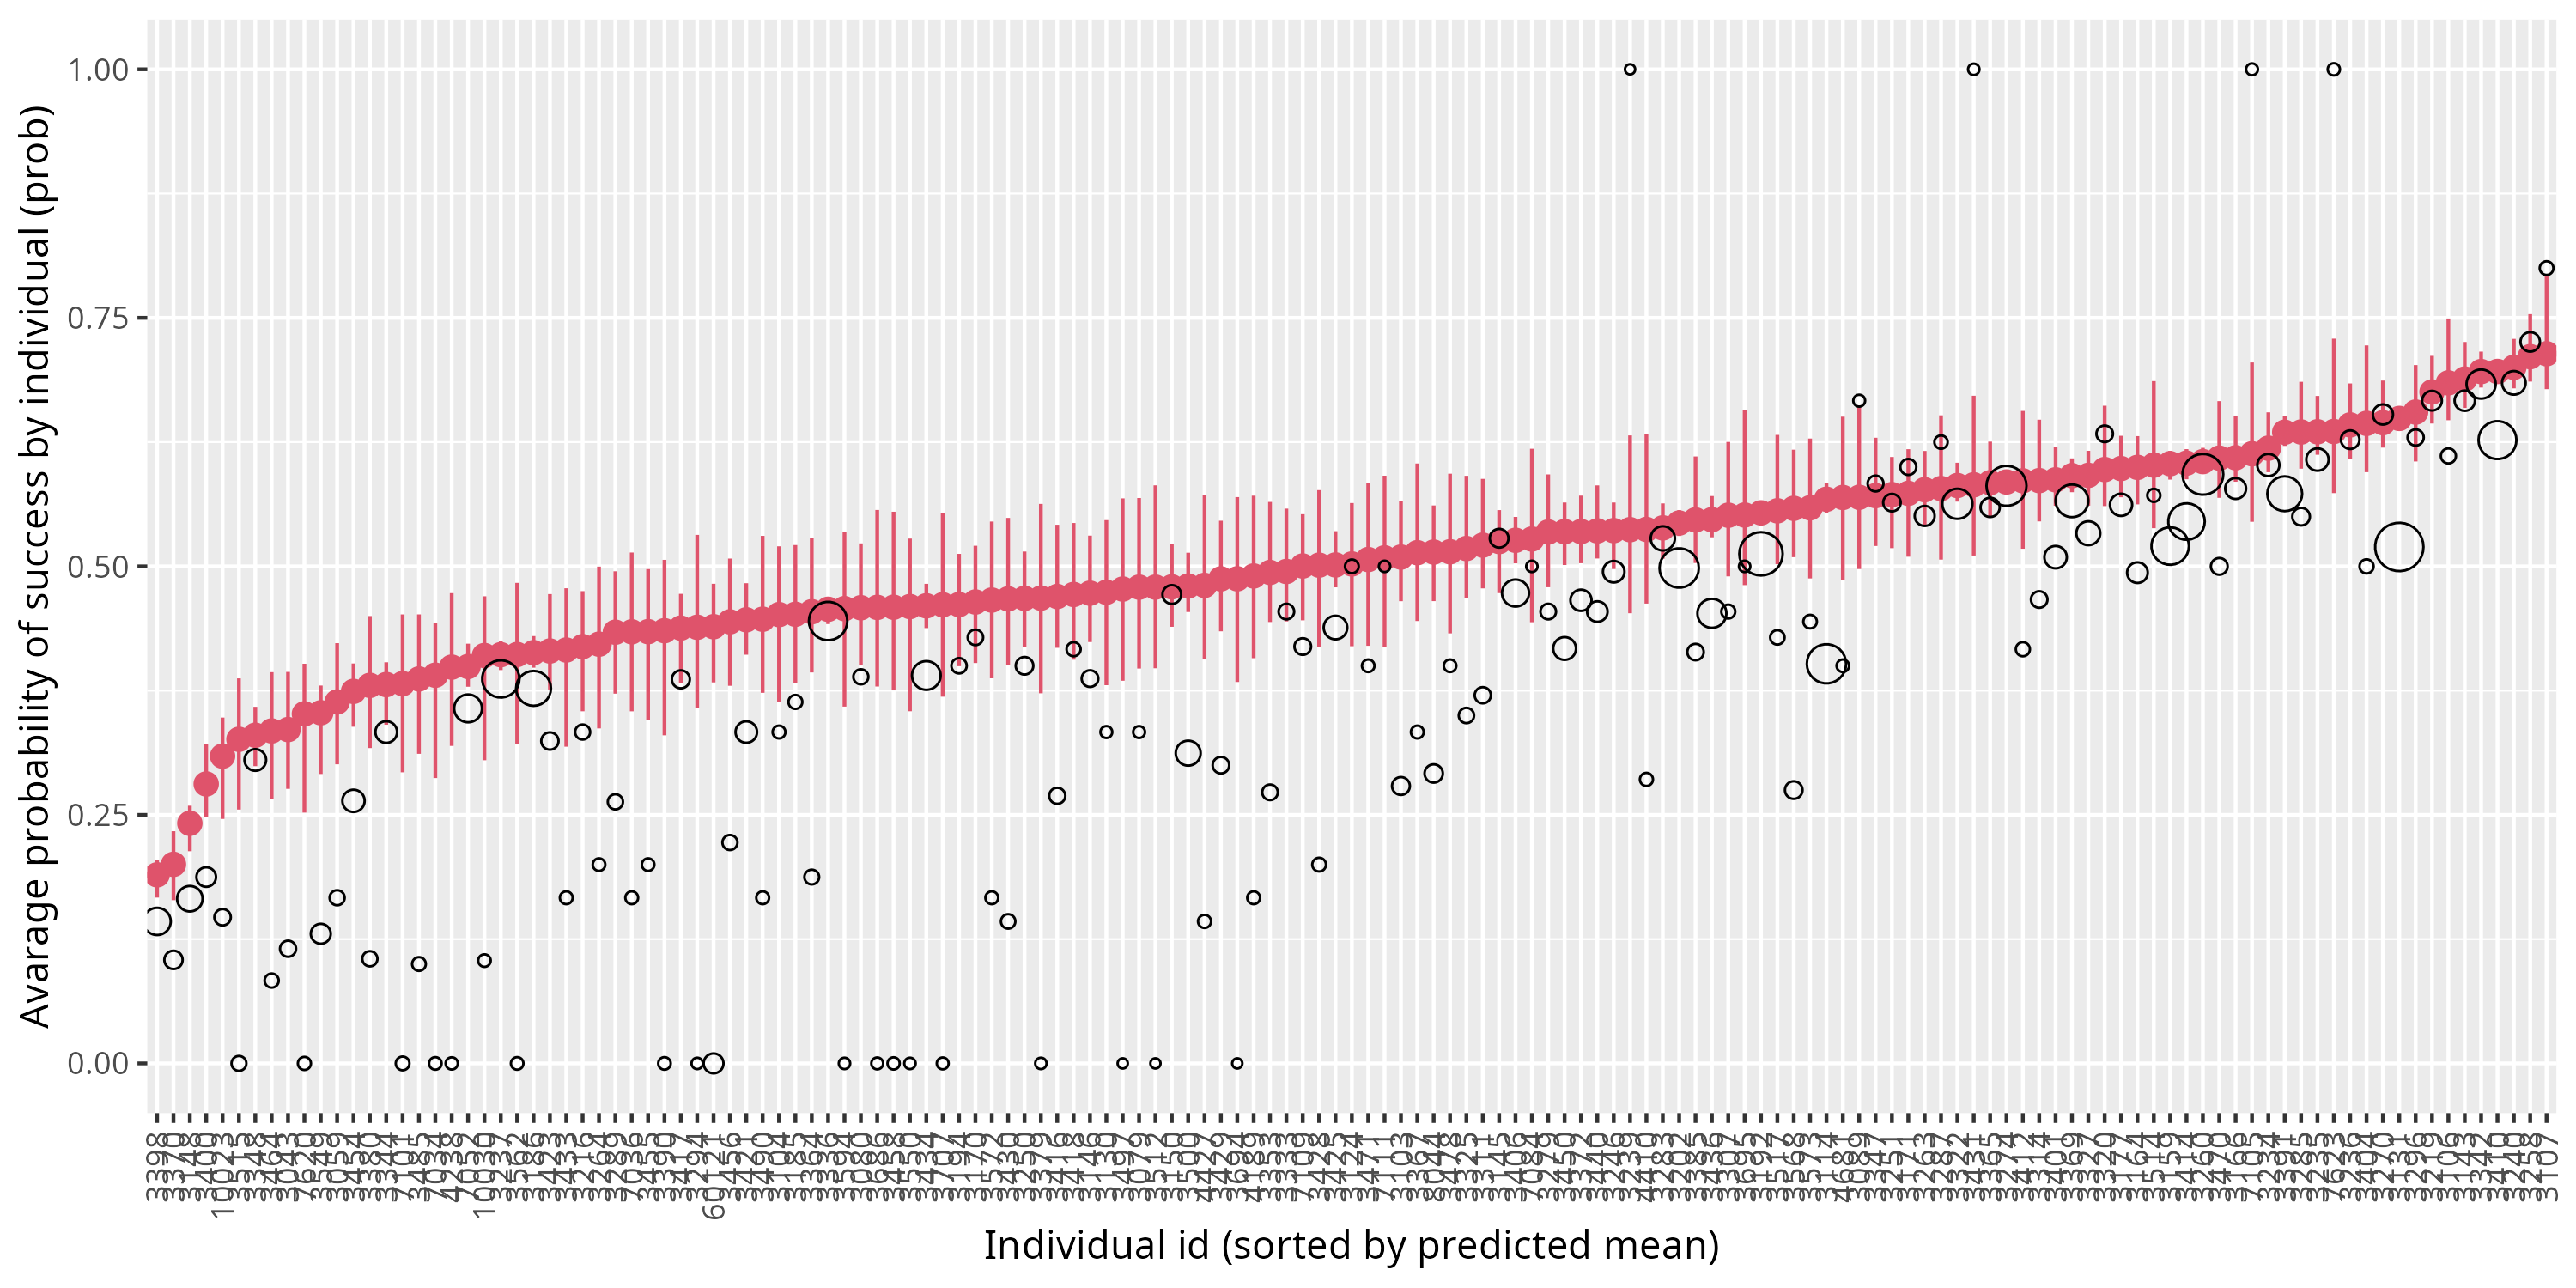
\includegraphics[width=0.80\textwidth]{./plots/p.posterior.mAI.4.png}
\end{center}
\caption{Posterior predictive distribution, marginalized over age ($A=0$ in the link function). The number of documented hunting trips per age is represented by the size of the points. The curve indicates the mean of the predictive posterior distribution with the 50\% HPDI compatibility interval.}\label{fig:p.posterior.mAI2}
\end{figure}

The variation of $\alpha$ and $\beta$ is described by the parameters $\sigma_\alpha$ and $\sigma_\beta$.
The mean variation of $\beta$ is slightly higher than that of $\alpha$, and it is itself subject to much more uncertainty, having a very long tail, see~\autoref{fig:sigma.posterior.mAI}.
This indicates that much of the variation is explained by the effect of the characteristics of the individuals on the chance of a hunting trip being successful.

\begin{figure}[htb!]
\begin{center}
    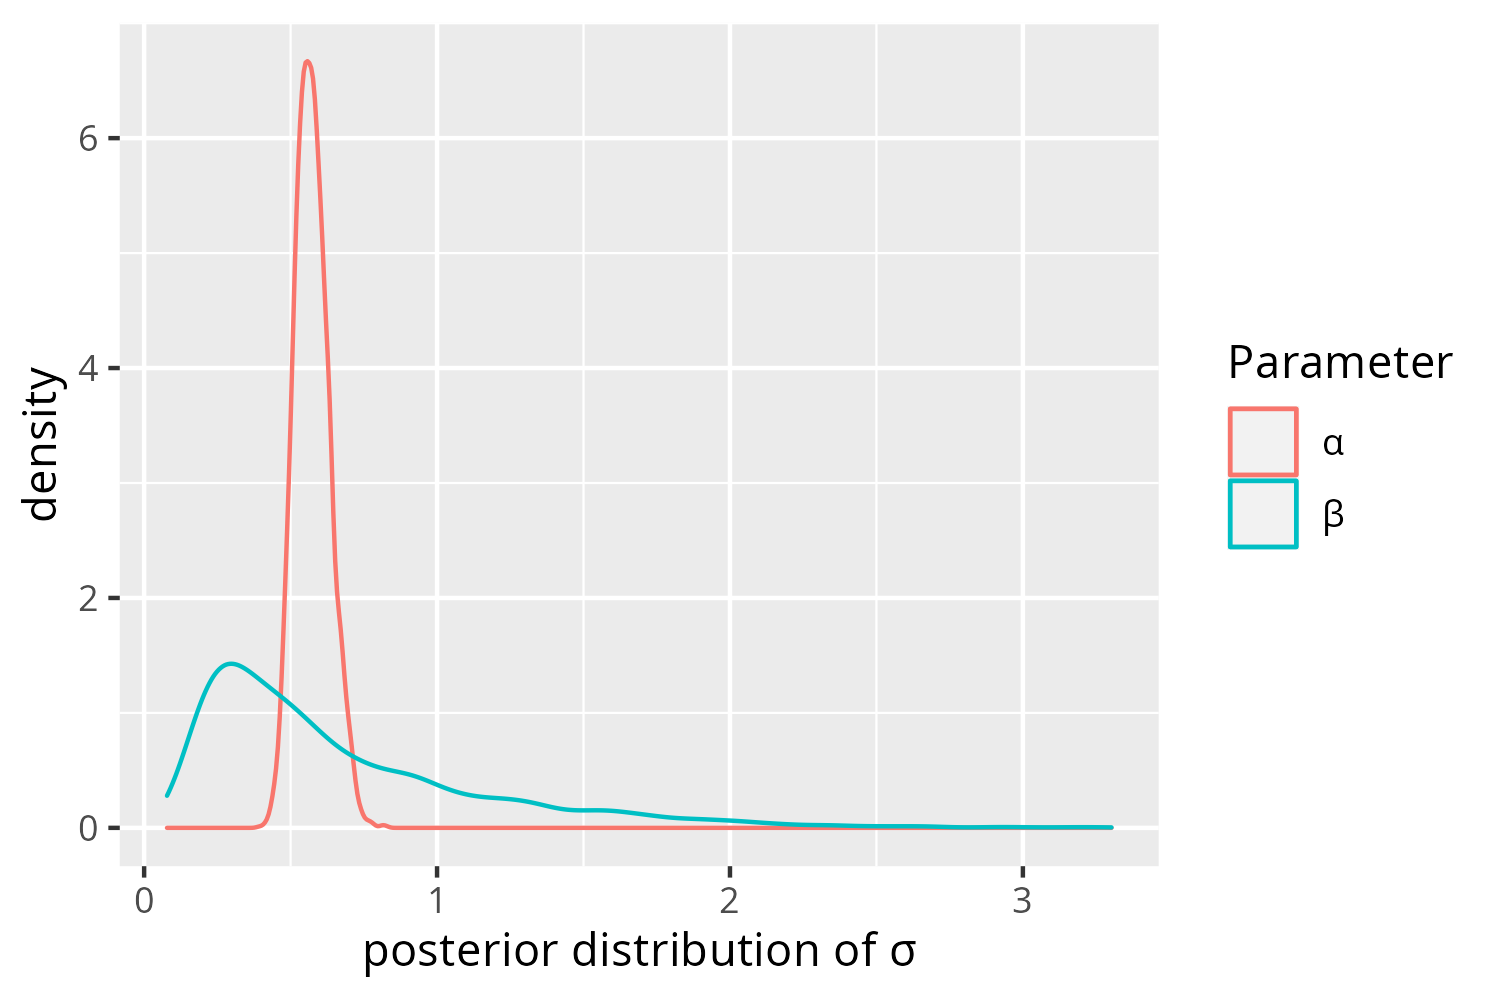
\includegraphics[width=0.75\textwidth]{./plots/sigma.posterior.mAI.png}
\end{center}
\caption{Posterior distribution of $\sigma_\alpha$ and $\sigma_\beta$.}\label{fig:sigma.posterior.mAI}
\end{figure}

\chapter*{Exercice 3}

\paragraph*{Complete cases}
To account for effect of the time taken for each trip on success on the complete cases, I assume that longer trips will give more opportunities for \emph{some} game to be scored, so I include a linear effect $\gamma$ over the time $T$.
In this model, the time taken for each trip is assumed to be independent of the hunters characteristics, believing that most of the variation is due to weather, luck and patterns of geographic distribution of the fauna being hunted.
To account for measurement errors of $T$, I include a submodel for $T_i$, that is a Normal distribution with mean on the average time taken for the recorded trips $\bar{T}$ and standard deviation $\sigma_T$.

\begin{alignat*}{2}
    T_i& \sim \normal(\bar{T}, \sigma_T)\\
    \sigma_T& \sim \exponential(1)
\end{alignat*}

The full model is as follows:

\begin{alignat*}{2}
    S_i& \sim \bernoulli(p_i)&\\
    \logit(p_i)& = \alpha_{H_i} + \beta A_i^2 + \gamma T_i\\
    \\
    T_i& \sim \normal(\bar{T}, \sigma_T)\\
    \sigma_T& \sim \exponential(1)&\\
    \\
    \alpha_j& = \bar{\alpha} + z_{\alpha,j}\sigma_\alpha{}& \text{for $j = 1 \dots 147$}\\
    z_{\alpha,j}& \sim \normal(0,1)&\\
    \bar{\alpha}& \sim \normal(0, 0.1)&\\
    \beta& = z_{\beta}\sigma_\beta&\\
    z_{\beta}& \sim \normal(0,1)&\\
    \gamma& \sim \normal(0,1)\\
    \sigma_\alpha, \sigma_\beta& \sim \exponential(1)&\\
\end{alignat*}

The model is processed by \texttt{ulam} and stored in a model file \texttt{models/mAITc.rds}:

\lstinputlisting[language=R, firstline=90, lastline=105]{./Geraldes-week9.R}

\paragraph*{Incomplete cases}
To account for effect of the time taken for each trip on success on the incomplete cases, the assumptions are the same as in the previous model.
The difference is in the submodel for $T_i$, that now has the work of imputing values for $T$.
We must not use the value for $\bar{T}$ directly in the normal distribution of $T_i$, as the real mean is unknown, so we derive a mean $\mu_T$ from another normal distribution with mean on the complete cases $\bar{T}$:

\begin{alignat*}{2}
    T_i& \sim \normal(\mu_T, \sigma_T)\\
    \mu_T& \sim \normal(\bar{T}, 1)\\
    \sigma_T& \sim \exponential(1)
\end{alignat*}

The full model is as follows:

\begin{alignat*}{2}
    S_i& \sim \bernoulli(p_i)&\\
    \logit(p_i)& = \alpha_{H_i} + \beta A_i^2 + \gamma T_i\\
    \\
    T_i& \sim \normal(\mu_T, \sigma_T)\\
    \mu_T& \sim \normal(\bar{T}, 1)\\
    \sigma_T& \sim \exponential(1)&\\
    \\
    \alpha_j& = \bar{\alpha} + z_{\alpha,j}\sigma_\alpha{}& \text{for $j = 1 \dots 147$}\\
    z_{\alpha,j}& \sim \normal(0,1)&\\
    \bar{\alpha}& \sim \normal(0, 0.1)&\\
    \beta& = z_{\beta}\sigma_\beta&\\
    z_{\beta}& \sim \normal(0,1)&\\
    \gamma& \sim \normal(0,1)\\
    \sigma_\alpha, \sigma_\beta& \sim \exponential(1)&\\
\end{alignat*}

The model is processed by \texttt{ulam} and stored in a model file \texttt{models/mAITi.rds}:

\lstinputlisting[language=R, firstline=119, lastline=135]{./Geraldes-week9.R}

\printbibliography{}

% \chapter*{Appendix: full code}

% \lstinputlisting[language=R]{./Geraldes-week9.R}

\end{document}
